% Options for packages loaded elsewhere
\PassOptionsToPackage{unicode}{hyperref}
\PassOptionsToPackage{hyphens}{url}
%
\documentclass[
  12pt,a4paper,lualatex,ja=standard]{bxjsarticle}
\usepackage{lmodern}
\usepackage{amsmath}
\usepackage{ifxetex,ifluatex}
\ifnum 0\ifxetex 1\fi\ifluatex 1\fi=0 % if pdftex
  \usepackage[T1]{fontenc}
  \usepackage[utf8]{inputenc}
  \usepackage{textcomp} % provide euro and other symbols
  \usepackage{amssymb}
\else % if luatex or xetex
  \usepackage{unicode-math}
  \defaultfontfeatures{Scale=MatchLowercase}
  \defaultfontfeatures[\rmfamily]{Ligatures=TeX,Scale=1}
\fi
% Use upquote if available, for straight quotes in verbatim environments
\IfFileExists{upquote.sty}{\usepackage{upquote}}{}
\IfFileExists{microtype.sty}{% use microtype if available
  \usepackage[]{microtype}
  \UseMicrotypeSet[protrusion]{basicmath} % disable protrusion for tt fonts
}{}
\makeatletter
\@ifundefined{KOMAClassName}{% if non-KOMA class
  \IfFileExists{parskip.sty}{%
    \usepackage{parskip}
  }{% else
    \setlength{\parindent}{0pt}
    \setlength{\parskip}{6pt plus 2pt minus 1pt}}
}{% if KOMA class
  \KOMAoptions{parskip=half}}
\makeatother
\usepackage{xcolor}
\IfFileExists{xurl.sty}{\usepackage{xurl}}{} % add URL line breaks if available
\IfFileExists{bookmark.sty}{\usepackage{bookmark}}{\usepackage{hyperref}}
\hypersetup{
  hidelinks,
  pdfcreator={LaTeX via pandoc}}
\urlstyle{same} % disable monospaced font for URLs
\usepackage{graphicx}
\makeatletter
\def\maxwidth{\ifdim\Gin@nat@width>\linewidth\linewidth\else\Gin@nat@width\fi}
\def\maxheight{\ifdim\Gin@nat@height>\textheight\textheight\else\Gin@nat@height\fi}
\makeatother
% Scale images if necessary, so that they will not overflow the page
% margins by default, and it is still possible to overwrite the defaults
% using explicit options in \includegraphics[width, height, ...]{}
\setkeys{Gin}{width=\maxwidth,height=\maxheight,keepaspectratio}
% Set default figure placement to htbp
\makeatletter
\def\fps@figure{htbp}
\makeatother
\setlength{\emergencystretch}{3em} % prevent overfull lines
\providecommand{\tightlist}{%
  \setlength{\itemsep}{0pt}\setlength{\parskip}{0pt}}
\setcounter{secnumdepth}{5}
\usepackage{indentfirst}
\parindent = 1em
\usepackage{dcolumn}
\newcolumntype{.}{D{.}{.}{-1}}
\usepackage{caption}
\captionsetup[table]{name=表}
\captionsetup[figure]{name=図}
\usepackage{hyperref}
\pagestyle{empty}
\usepackage{multicol}
\usepackage{ascmac}
\setpagelayout*{top=10truemm,bottom=30truemm,left=10truemm,right=10truemm}
\usepackage{tikz}
\usetikzlibrary{arrows.meta,decorations,decorations.pathreplacing}
\usepackage{tabstackengine}
\usepackage{xcolor}
\usepackage{rotating}
\usepackage{txfonts}
\usepackage{fancybox}
\usepackage{dashbox}
\usepackage{tcolorbox}
\tcbuselibrary{theorems,skins}
\usepackage{siunitx}
\usepackage{framed}
\usepackage{enumerate}
\usepackage{lastpage}
\ifluatex
  \usepackage{selnolig}  % disable illegal ligatures
\fi

\author{}
\date{\vspace{-2.5em}}

\begin{document}

\renewcommand{\thefootnote}{}
\newcounter{kaunta}
\renewcommand{\thekaunta}{\arabic{kaunta}}
\newcommand{\kaunta}{\refstepcounter{kaunta}%
\thekaunta}
\def\question{\noindent\fbox{\large\makebox[1em]{\text{\kaunta}}} \hspace{1pt}}
\newcounter{skaunta}
\renewcommand{\theskaunta}{\arabic{skaunta}}
\newcommand{\skaunta}{\refstepcounter{skaunta}%
\theskaunta}
\def\squestion{(\text{\skaunta})\hspace{2.5pt}}
\newcommand{\maru}[1]{\raise0.2ex\hbox{\textcircled{\scriptsize{#1}}}}

\newgeometry{top=10truemm,bottom=10truemm,left=20truemm,right=20truemm}

\thispagestyle{empty}
\begin{center}
\phantom{empty}

\vspace{60truemm}

\hspace{4em} {\HUGE\gtfamily\bfseries 数\hspace{2em}学}\hspace{1em}{\large \gtfamily \bfseries ($\mathbf{1}$年)}\\
\vspace{84truemm}

{\large\gtfamily\bfseries 注\hspace{5em}意}

\end{center}

\centering
\begin{framed}
\begin{flushleft}
\begin{enumerate}[\Large \gtfamily 1]
  \item {\large 「開始」の合図があるまでは,開いてはいけません。}

  \item {\large 問題は\pageref{LastPage}ページまであります。}

  \item {\large 「開始」の合図があったら,まず,問題用紙・解答用紙に,組・番号と名前などを書きなさい。}

  \item {\large 答えは,すべて解答用紙に書きなさい。また、所定の欄に濃くはっきりと書きなさい。}

  \item {\large 「終了」の合図で,すぐ鉛筆をおき,解答用紙を裏返しにしなさい。}
\end{enumerate}
\end{flushleft}
\end{framed}

\vspace{14mm}

\begin{center}
{\large \underline{\hspace{30mm}組 \hspace{30mm}番 \hspace{15mm} 名前 \hspace{60mm}}}
\end{center}

\pagestyle{plain}
\pagenumbering{arabic}

\begin{flushleft}

\noindent\fbox{\large\makebox[1em]{\text{\refstepcounter{kaunta}%
\arabic{kaunta}}}} \hspace{1pt}空欄にあてはまる言葉や数字を答えなさい。

\begin{flushright}
\footnotesize{<知・技$2 \times 6$点>}
\end{flushright}

式$2x + 1 = 7 \cdots \raise 0.2ex\hbox{\textcircled{\scriptsize{1}}}$や$\dfrac{1}{3}x = -6 \cdots \raise 0.2ex\hbox{\textcircled{\scriptsize{2}}}$のように文字に代入する値によって、成り立ったり、成り立たなかったりする等式を$\fbox{\quad \raise 0.2ex\hbox{\textcircled{\scriptsize{\mbox{ア}}}} \quad}$という。また、$\raise 0.2ex\hbox{\textcircled{\scriptsize{\mbox{ア}}}}$を成り立たせる文字の値を、$\raise 0.2ex\hbox{\textcircled{\scriptsize{\mbox{ア}}}}$の$\fbox{\quad \raise 0.2ex\hbox{\textcircled{\scriptsize{イ}}} \quad}$という。また、$\raise 0.2ex\hbox{\textcircled{\scriptsize{ア}}}$の$\raise 0.2ex\hbox{\textcircled{\scriptsize{イ}}}$を求めることを方程式を$\fbox{\quad \raise 0.2ex\hbox{\textcircled{\scriptsize{ウ}}} \quad}$という。

式$\raise 0.2ex\hbox{\textcircled{\scriptsize{1}}}$と$\raise 0.2ex\hbox{\textcircled{\scriptsize{2}}}$を等式の性質を使って解くと、
\begin{multicols}{2}
$$
\begin{aligned}
2x + 1 &= 7 \\
\mbox{両辺から}&\fbox{\quad \raise 0.2ex\hbox{\textcircled{\scriptsize{\mbox{エ} \quad}}}}\mbox{をひくと} \\
2x &= 6 \\
\mbox{両辺を}&\fbox{\quad \raise 0.2ex\hbox{\textcircled{\scriptsize{\mbox{オ} \quad}}}}でわると \\
x &= 3
\end{aligned}
$$
\columnbreak

$$
\begin{aligned}
\dfrac{1}{3}x &= 6 \\
\mbox{両辺に}&\fbox{\quad \raise 0.2ex\hbox{\textcircled{\scriptsize{\mbox{カ} \quad}}}}\mbox{をかけると}\\
x &= 18
\end{aligned}
$$

\end{multicols}

\noindent\fbox{\large\makebox[1em]{\text{\refstepcounter{kaunta}%
\arabic{kaunta}}}} \hspace{1pt}次の方程式を解きなさい。

\begin{flushright}
\footnotesize{<知・技$2 \times 25$点>}
\end{flushright}

(\text{\refstepcounter{skaunta}%
\arabic{skaunta}})\hspace{2.5pt}$x - 7 = 6$ \hfill (\text{\refstepcounter{skaunta}%
\arabic{skaunta}})\hspace{2.5pt}$\dfrac{1}{2}x + 3 = x - 1$ \hfill (\text{\refstepcounter{skaunta}%
\arabic{skaunta}})\hspace{2.5pt}$3(x - 2) = 5x - 10$ \hfill (\text{\refstepcounter{skaunta}%
\arabic{skaunta}})\hspace{2.5pt}$x : 3 = 4 : 5$

\vspace{30mm}

(\text{\refstepcounter{skaunta}%
\arabic{skaunta}})\hspace{2.5pt}$2x + 9 = 5$\hfill (\text{\refstepcounter{skaunta}%
\arabic{skaunta}})\hspace{2.5pt}$2x + 5 = -3x + 10$ \hfill (\text{\refstepcounter{skaunta}%
\arabic{skaunta}})\hspace{2.5pt}$5x + 3 = 2(x - 9)$ 

\vspace{30mm}

(\text{\refstepcounter{skaunta}%
\arabic{skaunta}})\hspace{2.5pt}$\dfrac{2x - 1}{5} = \dfrac{x - 2}{4}$ \hfill (\text{\refstepcounter{skaunta}%
\arabic{skaunta}})\hspace{2.5pt}$0.005x + 1.2 = 0.16x - 1$ \hfill (\text{\refstepcounter{skaunta}%
\arabic{skaunta}})\hspace{2.5pt}$5 : 6 = 15 : x$ 

\vspace{30mm}

(\text{\refstepcounter{skaunta}%
\arabic{skaunta}})\hspace{2.5pt}$x : (14 -x) = 3 : 4$ \hfill (\text{\refstepcounter{skaunta}%
\arabic{skaunta}})\hspace{2.5pt}$-x + 8 = 3x$ \hfill (\text{\refstepcounter{skaunta}%
\arabic{skaunta}})\hspace{2.5pt}$12y + 1 = 9y + 5$

\newpage

(\text{\refstepcounter{skaunta}%
\arabic{skaunta}})\hspace{2.5pt}$3x - 4(2x - 1) = 29$ \hfill (\text{\refstepcounter{skaunta}%
\arabic{skaunta}})\hspace{2.5pt}$2(x - 1) = 7(- x - 8)$ \hfill (\text{\refstepcounter{skaunta}%
\arabic{skaunta}})\hspace{2.5pt}$1.3 - 0.8x = 0.9 - x$ 

\vspace{30mm}

(\text{\refstepcounter{skaunta}%
\arabic{skaunta}})\hspace{2.5pt}$\dfrac{3}{2}a - 7 = \dfrac{1}{3}a$ \hfill (\text{\refstepcounter{skaunta}%
\arabic{skaunta}})\hspace{2.5pt}$0.3(0.2x - 1) = 0.54$ \hfill (\text{\refstepcounter{skaunta}%
\arabic{skaunta}})\hspace{2.5pt}$\dfrac{2}{3}x -3 = \dfrac{1}{12}(3x + 4)$

\vspace{30mm}

(\text{\refstepcounter{skaunta}%
\arabic{skaunta}})\hspace{2.5pt}$(x + 1):3 = 5x :12$ \hfill (\text{\refstepcounter{skaunta}%
\arabic{skaunta}})\hspace{2.5pt}$3x = 21$ \hfill (\text{\refstepcounter{skaunta}%
\arabic{skaunta}})\hspace{2.5pt}$17x = -17$ 

\vspace{30mm}

(\text{\refstepcounter{skaunta}%
\arabic{skaunta}})\hspace{2.5pt}$18 = -2x$ \hfill (\text{\refstepcounter{skaunta}%
\arabic{skaunta}})\hspace{2.5pt}$\dfrac{x}{7} = 3$ \hfill (\text{\refstepcounter{skaunta}%
\arabic{skaunta}})\hspace{2.5pt}$\dfrac{4x -5}{3} = 2x - 9$

\vspace{30mm}

\newpage

\begin{multicols}{2}
\noindent\fbox{\large\makebox[1em]{\text{\refstepcounter{kaunta}%
\arabic{kaunta}}}} \hspace{1pt}
正さんは、右の方程式の解き方がまちがっていることに気づきました。アからウのどこで$\underline{\mbox{初めてまちがえていますか}}$。初めてまちがえている式の記号を書きなさい。また、この方程式の正しい解を求めなさい。

\begin{flushright}
\footnotesize{<知・技$3 \times 2$点>}
\end{flushright}

\columnbreak
\begin{screen}
\begin{align*}
5x - 2 &= 7x + 10 \\
5x + 7x &= 10 + 2  &\cdots \mbox{ア}\\
12x &= 12 &\cdots \mbox{イ}\\
x &= 0 &\cdots \mbox{ウ}
\end{align*}
\end{screen}
\end{multicols}

\vfill

\noindent\fbox{\large\makebox[1em]{\text{\refstepcounter{kaunta}%
\arabic{kaunta}}}} \hspace{1pt}$x$についての方程式$5x + 5 = 3x -4a$の解が$-3$であるとき、$a$の値を求めなさい。
\begin{flushright}
\footnotesize{<知・技5点>}
\end{flushright}

\vfill

\newpage

\setcounter{skaunta}{0}
\noindent\fbox{\large\makebox[1em]{\text{\refstepcounter{kaunta}%
\arabic{kaunta}}}} \hspace{1pt}1本150円のジュースを何本かと、200円のお菓子を1個買ったら、代金の合計が140円でした。このとき、次の問に答えなさい。

\begin{flushright}
\footnotesize{<知・技$5 \times 2$点>}
\end{flushright}


(\text{\refstepcounter{skaunta}%
\arabic{skaunta}})\hspace{2.5pt}ジュースを$x$本買ったとして、ジュースの本数を求めるための方程式をつくりなさい。

\vfill

(\text{\refstepcounter{skaunta}%
\arabic{skaunta}})\hspace{2.5pt}(1)で作った方程式を解いて、ジュースの本数を求めなさい。

\vfill

\noindent\fbox{\large\makebox[1em]{\text{\refstepcounter{kaunta}%
\arabic{kaunta}}}} \hspace{1pt}ウスターソースとケチャップを$2 : 3$の割合で混ぜて、ハンバーグソースを作ります。
ケチャップを$120 \si{ml}$使うとき、ウスターソースは何$\si{ml}$あればよいでしょうか。<知・技5点>

\vfill
\vfill

\newpage

\setcounter{skaunta}{0}
\noindent\fbox{\large\makebox[1em]{\text{\refstepcounter{kaunta}%
\arabic{kaunta}}}} \hspace{1pt}武さんは、ケーキがすべて同じ値段で販売されるセールに出かけ、おばあちゃんの家に持っていくお土産のケーキを買ってきました。武さんは、次のように言っています。

\begin{flushright}
\footnotesize{<(1)思・判・表$5 \times 2$点、(2)思・判・表6点>}
\end{flushright}

\begin{figure}[h]
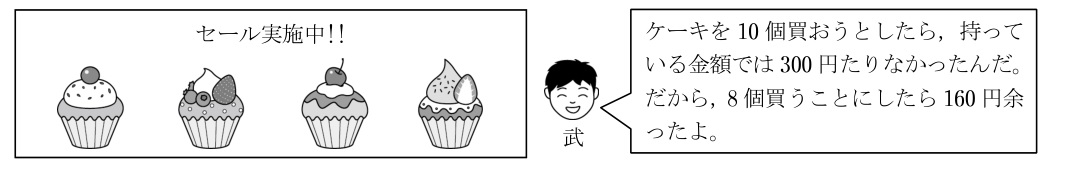
\includegraphics[height=30truemm]{cake.jpg}
\end{figure}

\begin{multicols}{2}
(\text{\refstepcounter{skaunta}%
\arabic{skaunta}})\hspace{2.5pt}武さんが持っている金額は、右のようにして求めることができます。

右の\doublebox{\qquad\phantom{250円}}に、武さんが持っている式を書き、問題の答えを求めなさい。

\columnbreak
\begin{screen}
ケーキ1個の値段を$x$円とすると
\begin{align*}
10x - 300 &= 8x + 160 \\
2x &= 460 \\
x &= 230
\end{align*}
したがって、武さんが持っている金額は

\hspace*{25mm}\doublebox{\qquad \phantom{250円}}

これは、問題に適している。
\begin{flushright}
$\underline{\mbox{答 }\fbox{\quad\phantom{250}}\mbox{円}}$
\end{flushright}
\end{screen}

\end{multicols}

(\text{\refstepcounter{skaunta}%
\arabic{skaunta}})\hspace{2.5pt}(1)で、武さんが持っている金額を求めた方法は、次のように説明できます。

\begin{screen}
ケーキ1個の値段を$x$円とし、武さんが持っている金額に着目して方程式をつくり、$x$の値を求め、方程式の左辺または右辺に$x$の値を代入して、持っている金額を求める。
\end{screen}

この問題は、方程式$\dfrac{x + 300}{10} = \dfrac{x -160}{8}$を解くことでも、武さんが持っている金額を求めることができます。その方法を、上にならって説明しなさい。

\vfill

\end{flushleft}

\end{document}
